\section{VMware} \label{section: VMware}

VMware is a company that specializes in developing technologies for virtualization and cloud computing. Its software products and services enable organizations to efficiently manage their IT infrastructure, improve performance, and reduce costs. VMware offers solutions for network virtualization, cloud management, digital workspace solutions, and security solutions.

\subsection{vSphere 6.5}
vSphere is VMware's virtualization software suite that allows you to create and manage virtual machines and computing environments, using a set of software tools and services. With vSphere, you can run multiple virtual machines on the same physical server, each running its own operating system and applications. vSphere includes many features and capabilities that help make virtualized environments more reliable, scalable, and performant, such as: 

\begin{itemize}
    \item \textbf{vSphere Web Client}: A web-based management interface. 
    \item \textbf{ESXi}: The bare metal hypervisor installed on your machines. 
    \item \textbf{vCenter}: A centralized management system for your vSphere environment.
    \item \textbf{vSAN}: A software-defined storage solution to create a distributed storage platform in vSphere.
    \item \textbf{NSX}: A software-defined networking solution for your vSphere environment.
    \item \textbf{VMotion:} Software to migrate VMs between servers without interruption of service.
\end{itemize}

\subsection{vSphere Web Client}
The \href{https://docs.vmware.com/en/VMware-vSphere/7.0/com.vmware.vsphere.vcenterhost.doc/GUID-A618EF76-638A-49DA-991D-B93C5AC0E2B1.html}{vSphere Client} is an application that enables administrators to manage and monitor VMware vSphere environments. It comes with a graphical user interface (GUI) and allows users to connect to VMware vCenter Server, which serves as a central management console for multiple VMware vSphere hosts.

Through the vSphere Client, administrators can create and modify virtual machines, manage storage, configure networking, and monitor system performance, among other things. Essentially, it provides a range of tools that enable users to manage virtual infrastructure components effectively. In addition to the traditional Windows-based vSphere Client, there's also a web-based version called the vSphere Client (HTML5), which is designed to work seamlessly across different operating systems and devices, including desktops, laptops, and mobile devices. This new client offers a simplified interface, improved performance, and support for new features introduced in vSphere 6.5 and later versions.

\begin{figure}[H]
    \centering
    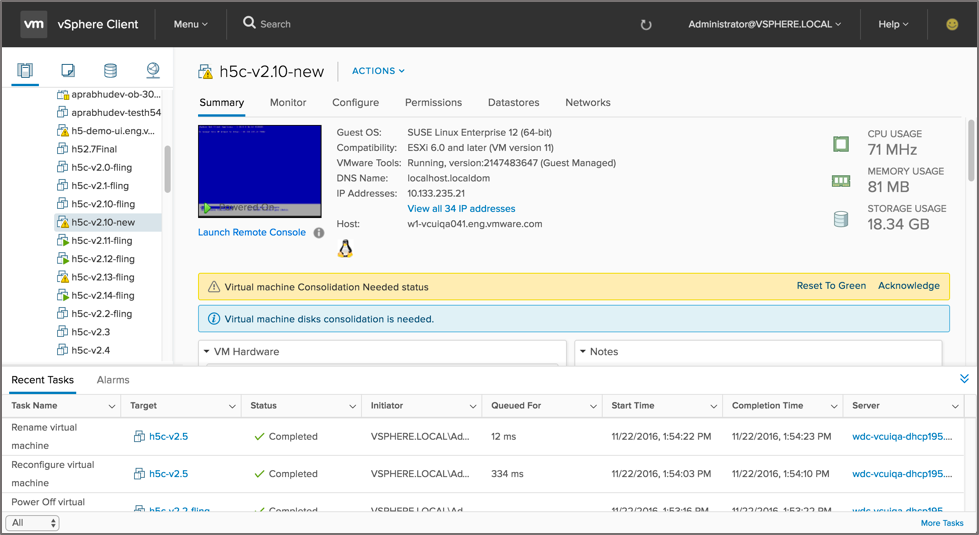
\includegraphics[scale = 0.9]{images/vsphere-client.jpg}
    \caption{vSphere Client \textcolor{red}{(STOLEN EXAMPLE)} }
    \label{vSphere Client}
\end{figure}

\subsection{ESXi}
VMware ESXi formerly known as ESX is a bare metal hypervisor that is installed directly on the physical server hardware and provides the ability to create, run, and manage virtual machines.

\begin{figure}[H]
    \centering
    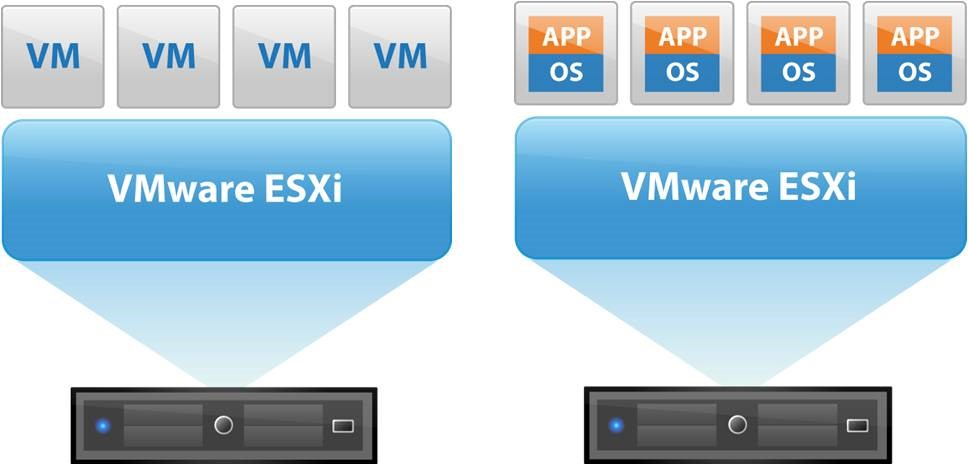
\includegraphics[scale = 0.55]{images/esxi.jpg}
    \caption{ESXi \textcolor{red}{(STOLEN EXAMPLE)} }
    \label{ESXi}
\end{figure}

\subsection{vCenter}
vCenter is a software platform that provides centralized management and control for their suite of virtualization products, including vSphere. By providing a single point of control, it simplifies management and reduces complexity, making it easier to manage many virtual machines and components. With vCenter, you can manage hosts, clusters, virtual machines, networks, and storage resources to support a virtualized environment with high availability, disaster recovery, and workload balancing.

In addition, vCenter provides advanced capabilities like automation, orchestration, and policy-based management. These features allow you to automate routine tasks, streamline operations, and enforce policies across your virtualized environment. Examples of automated tasks include: provisioning VMs \footnote{Create new virtual machines, configure virtual hardware, and install operating systems and applications.}, patches and updates \footnote{Deploy software updates, apply security patches, and performing maintenance tasks.}, backup and recovery \footnote{Create backup schedules, perform backup and restore operations, and monitor backup performance.}, monitor and reports \footnote{Generate reports on virtual machine performance, track resource usage, and monitor system health.}, and resource allocation \footnote{Adjust CPU and memory resources, configure storage allocations, and manage network bandwidth.}.

\begin{figure}[H]
    \centering
    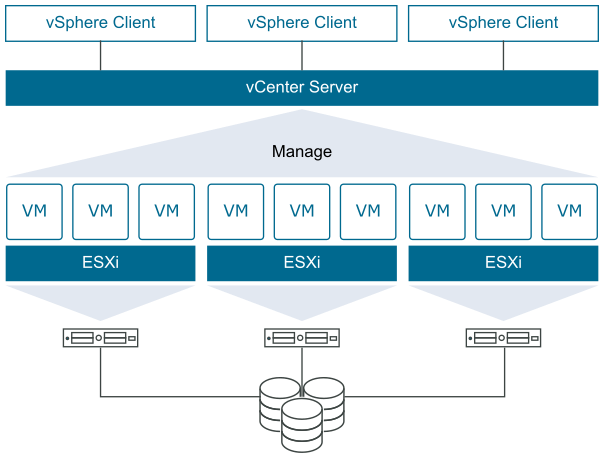
\includegraphics[scale = 0.65]{images/vmware-infrastructure-relationship.png}
    \caption{vCenter \textcolor{red}{(STOLEN EXAMPLE)} }
    \label{vCenter}
\end{figure}

\subsubsection{vCenter Security and Risks}
Security is a critical aspect of virtualized environments, and vCenter provides a range of security features to protect against unauthorized access, data theft, and data manipulation. These security features include: role-based access control\footnote{Define roles and permissions to users based on their roles to prevent unauthorized access.}, auditing\footnote{Track user activity and changes to identify security issues and log actions taken within the virtualized environment.}, encryption\footnote{Encrypt VM data, configuration files, and communication between hosts.}, secure communication\footnote{Supports SSL/TLS encryption to secure communication between hosts and the vCenter server.}, integration\footnote{Integrate with third-party security products (e.g., antivirus, IDS) to provide additional layers of security}, and two-factor authentication\footnote{Provide two forms of identification before accessing the VM to prevent unauthorized access.}. These security features help to ensure confidentiality, integrity, and availability of the virtualized infrastructure, a requirement when working with PHI data. 

\subsection{vSAN}
\href{https://docs.vmware.com/en/VMware-vSphere/7.0/com.vmware.vsphere.vsan-planning.doc/GUID-A80526C8-A941-4F84-9D44-D4B8B3914A95.html}{vSAN} is a software-defined storage solution developed by VMware, which allows organizations to create a distributed storage platform that is integrated with vSphere. This provides a highly scalable and available storage infrastructure, using standard hardware.

By creating a shared data store using the internal disks of ESXi hosts in a vSphere cluster, vSAN allows organizations to pool their storage capacity and performance into a single datastore, scaling it easily by adding more hosts to the cluster. vSAN features data replication, erasure coding, and automatic data rebalancing. Additionally, it offers advanced storage services such as deduplication, compression, and encryption, ensuring optimal storage efficiency and security which streamlines storage management, automates routine tasks, and helps to optimize storage utilization and cost savings.

\begin{figure}[H]
    \centering
    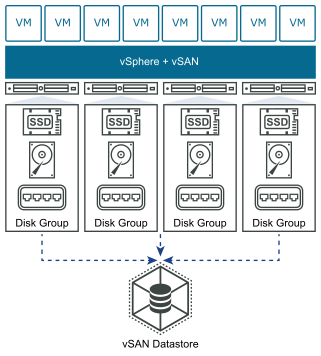
\includegraphics[scale = .8]{images/vsan-deployment.png}
    \caption{Standard vSAN Cluster \textcolor{red}{(STOLEN EXAMPLE)} }
    \label{vSan}
\end{figure}

\subsection{NSX}
\href{https://docs.vmware.com/en/VMware-NSX/index.html}{NSX} is a network virtualization and security platform created by VMware that provides a software-defined networking (SDN) solution that enables organizations to virtualize their network infrastructure, creating a more flexible, scalable, and manageable network.

NSX allows for all network components in your infrastructure to be virtualized, decoupling your network from existing hardware. This abstraction enables organizations to pool and automate network resources, which can reduce the time and cost of deploying and managing network infrastructure. NSX also offers advanced security features and networking capabilities which allows administrators to apply precise policies to specific workloads or applications. For example, NSX provides: network automation, multi-cloud and on-premises support, network segmentation, minimal cost and resource overhead, switching and routing, and load balancing features. 

\begin{figure}[H]
    \centering
    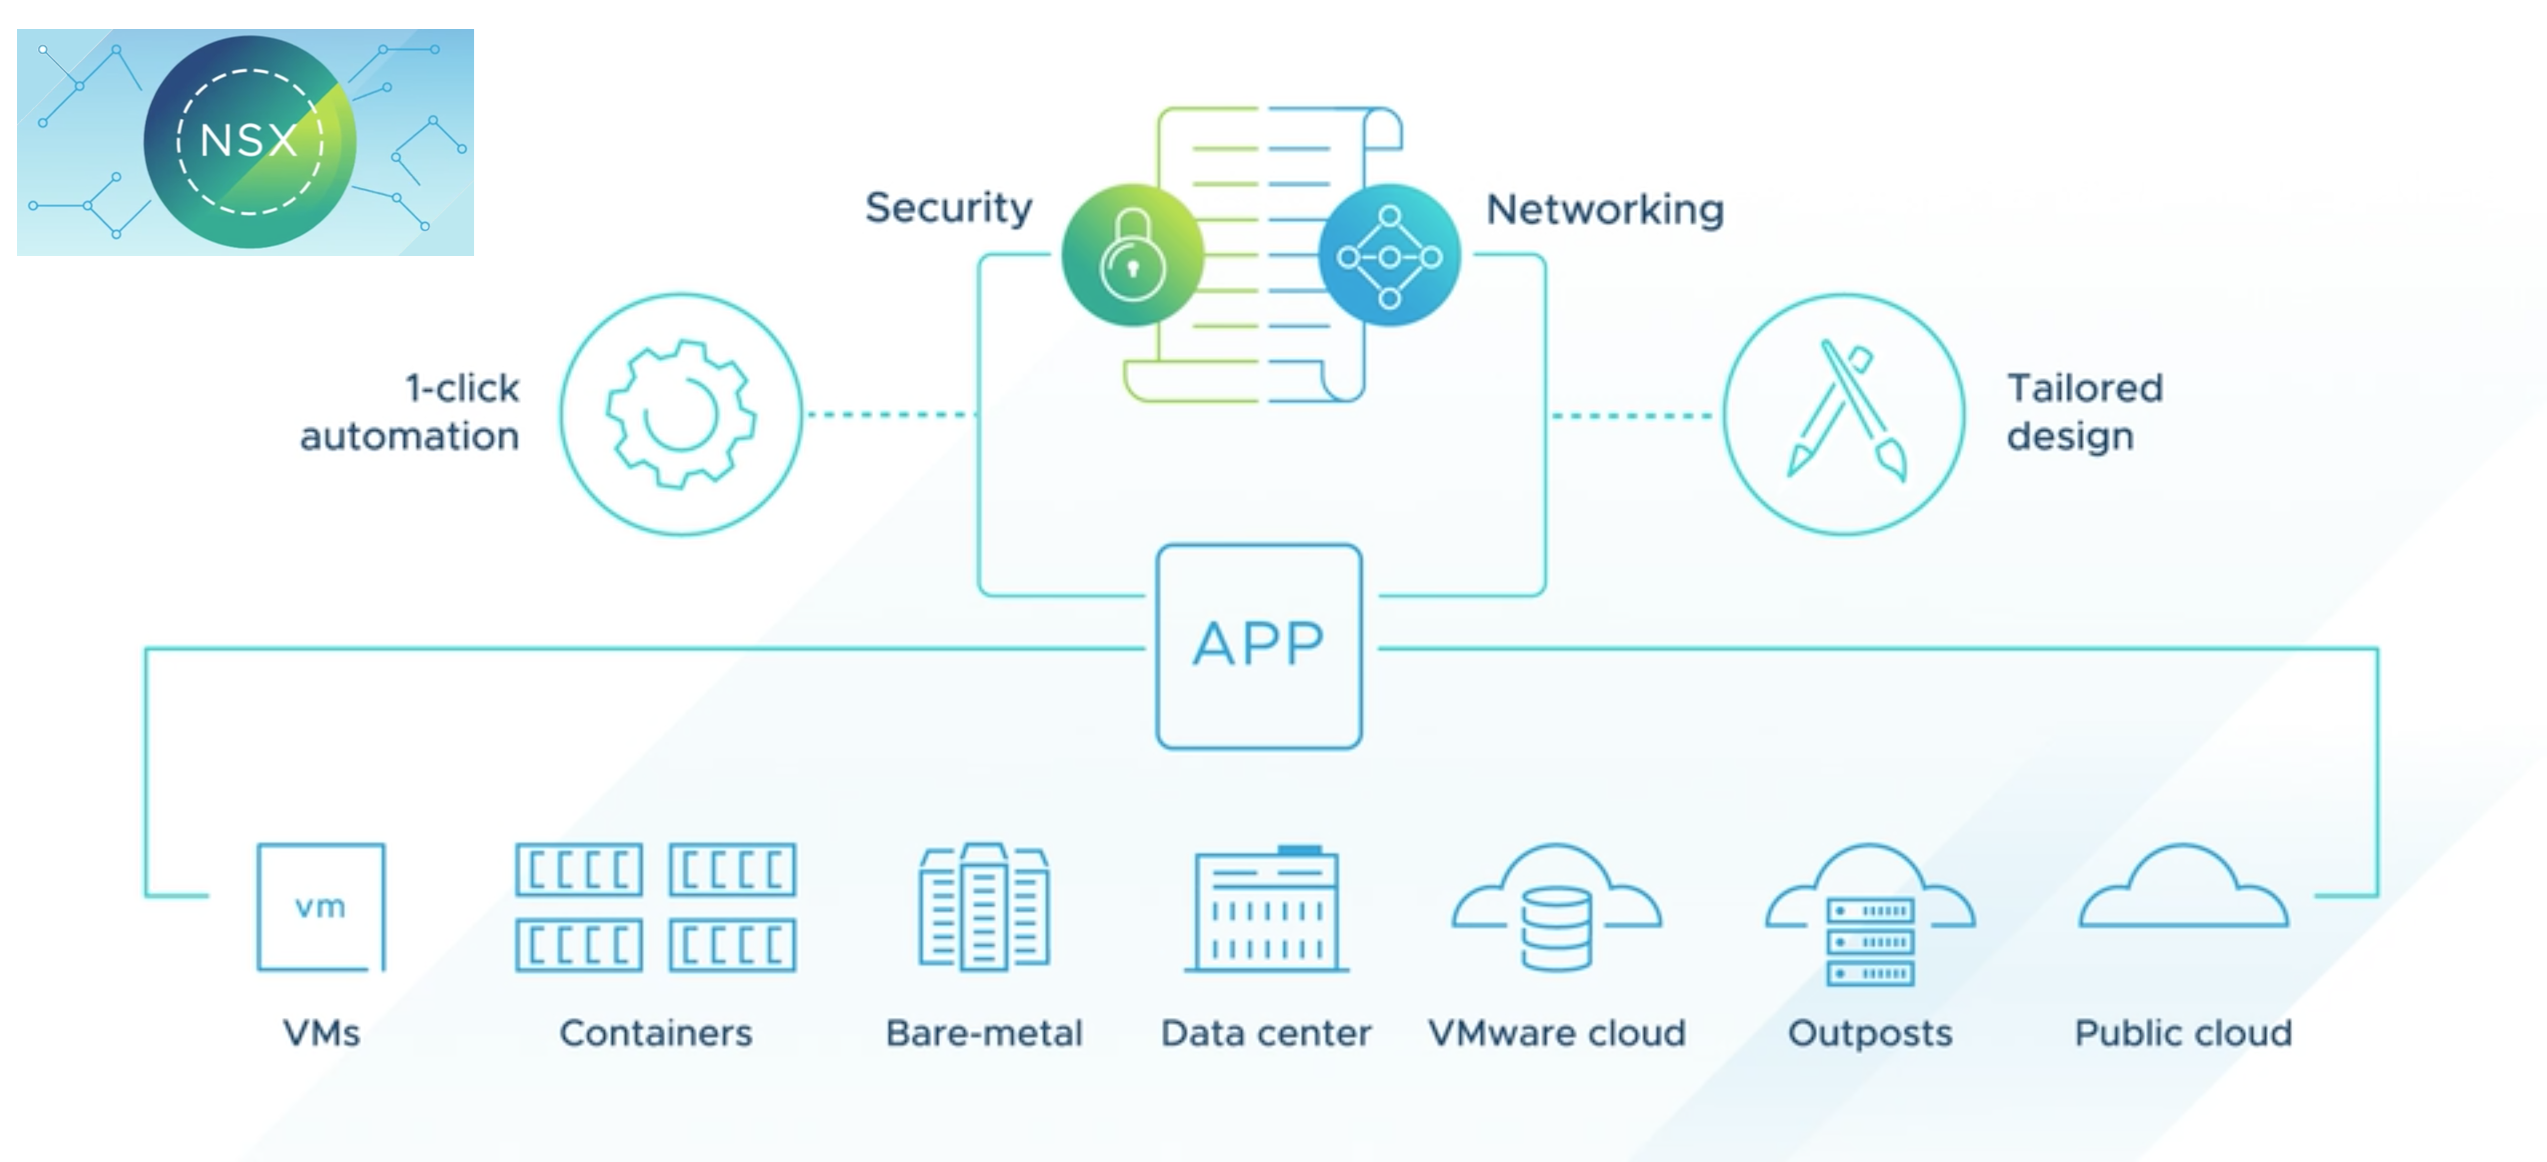
\includegraphics[scale = .19]{images/nsx-diagram.png}
    \caption{NSX Infrastructure \textcolor{red}{(STOLEN EXAMPLE)} }
    \label{NSX}
\end{figure}

\subsection{VMotion}
\href{https://www.vmware.com/products/vsphere/vmotion.html#:~:text=vMotion%20allows%20you%20to%3A,a%20virtual%20machine%20in%20seconds}{VMotion} is virtualization software that enables IT administrators to move VMs between physical servers or hosts without disrupting service. The process involves copying the entire state of the VM, including memory, CPU state, and network connections, from one host to another. The benefits of VMotion include increased availability and uptime, improved hardware utilization, workload balancing, and reduced downtime for maintenance and upgrades. However, the feature also requires specialized hardware and software, increasing the complexity of virtualized environments. VMotion uses shared storage, high-speed networking, and specialized software to ensure a seamless migration. 

The main use case for VMotion is to provide high availability and workload balancing for virtualized environments by optimizing resource usage, improving performance, and avoiding downtime during maintenance or upgrades. For example, an IT administrator can use VMotion to move running VMs to another host during server maintenance, ensuring uninterrupted service for end-users. Once the maintenance is complete, the VMs can be moved back to the original host. VMotion also allows for the consolidation of workloads and the migration of VMs to new hosts for improved hardware utilization and cost savings.

When migrating VMs with sensitive data, such as protected health information (PHI), there may be compliance issues with regulations like HIPAA. To ensure compliance, virtualization infrastructure and VMotion must be configured to meet data protection, access control, and auditability requirements. Encryption and other security measures should also be implemented to protect the confidentiality, integrity, and availability of PHI during migration. IT administrators should ensure that host servers and network connections used for VMotion are secure and protected from unauthorized access.

\begin{figure}[H]
    \centering
    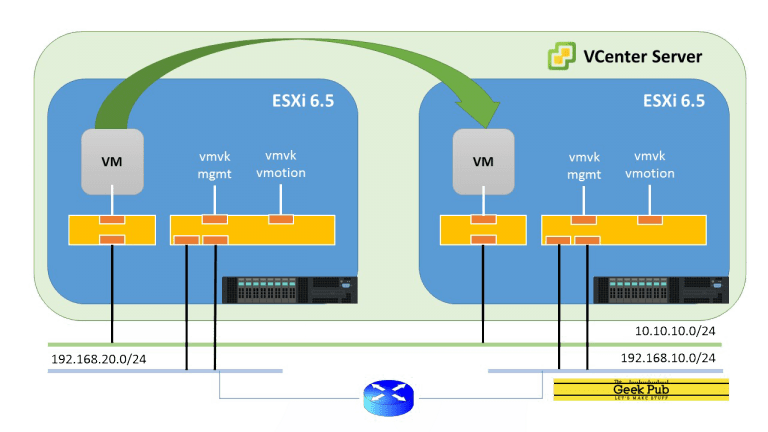
\includegraphics[scale = .50]{images/vmotion.png}
    \caption{VMotion \textcolor{red}{(STOLEN EXAMPLE)} }
    \label{VMotion}
\end{figure}